\documentclass[letterpaper, 12 pt]{article}

% The following packages can be found on http:\\www.ctan.org
\usepackage{graphics} % for pdf, bitmapped graphics files
\usepackage[pdftex]{graphicx}
\usepackage{multicol}
\usepackage{amsthm}
\usepackage{subcaption}
\usepackage{mathtools}
\DeclarePairedDelimiter{\ceil}{\lceil}{\rceil}
\usepackage{epsfig}   % for postscript graphics files
% \usepackage{mathptmx} % assumes new font selection scheme installed
\usepackage{times}    % assumes new font selection scheme installed
\usepackage{amsmath}  % assumes amsmath package installed
\usepackage{amssymb}  % assumes amsmath package installed
\usepackage{tikz}
\usepackage{fancyhdr}
\usetikzlibrary{arrows.meta}
% \usepackage{eucal} %gives a slightly curlier font than the default; changes the font that is 
% selected by 
% \mathcal

\usepackage{fancyhdr}
\usepackage[margin=2cm]{geometry}
\usepackage{graphicx}
\usepackage{graphics}
\usepackage{hyperref}
\usepackage{psfrag}
\usepackage{ifthen}
\usepackage{array}
\usepackage{longtable}
\usepackage{color}
\usepackage{tikz}
\usetikzlibrary{arrows.meta}
\usepackage{bm}
\usepackage{amsmath, amsfonts}
\usepackage[shortlabels]{enumitem}
\setcounter{secnumdepth}{0}

\setlength{\textwidth}{6.5in}
\setlength{\oddsidemargin}{-0.1in}
\setlength{\evensidemargin}{-0.1in}
% 1in on top and bottom
\setlength{\headheight}{0.1in}
\setlength{\headsep}{0.2in}        %{15pt=0.207555in}
\setlength{\footskip}{0.2in}         %{30pt=0.41511in}
\setlength{\textheight}{9.0in}
\setlength{\hoffset}{0in}
\setlength{\voffset}{0pt}
\setlength{\topmargin}{-0.5in}
\setlength{\parskip}{5pt plus5pt minus5pt}
\setlength{\parindent}{0in}
\renewcommand{\baselinestretch}{1.25}
\usepackage{titling}
\newcommand{\subtitle}[1]{%
    \posttitle{%
    \par\end{center}
    \begin{center}\large#1\end{center}
        \vskip0.5em}%
        }

        \newtheorem{definition}{Definition}
        \newcommand{\ds}{\displaystyle}
        \newcommand{\p}{\partial}
        \newcommand{\R}{\text{I\!R}}
        \newcommand{\HRule}{\rule{\linewidth}{0.5mm}}
\def\endproof{\begin {flushright}$\text{gg ez } \blacksquare$ \end{flushright}}

\fancyhead{}
\fancyhead[R]{CWID: 103-99-961}
\fancyhead[L]{Homework 3}
\fancyhead[C]{Hayden Pott}
\renewcommand\headrulewidth{0pt}
\fancyfoot{}
\fancyfoot[C]{\thepage}

\pagestyle{fancy}

\begin{document}
\begin{center}
    \Large CSC 310\\
    Homework 3\\
    \normalsize
    14 May 2024\\

    Some work with Landen Nguyen
\end{center}

\Large \textbf{Lecture 11}

\normalsize

\begin{enumerate}
    \item[1.] [True or False] Determining whether two transition graphs define
        the same language is decidable. \\
        \textbf{ANS:} True

    \item[2.] [True or False] Determining whether two NFA’s define the same
        language is decidable.\\
        \textbf{ANS:} True

    \item[3.] [True or False] Every Regular Language is a Context Free Language.
        \\
        \textbf{ANS:} True

    \item[4.] Refer back to Example 2 on Slide 10 of this lecture (Lecture 11).
        Provide a derivation for the word “aaabb” using the annotated version of
        the standard derivation format (also presented on Slide 10). \\
        \textbf{ANS:} \\
        $
        \underline{S} \overset{1}{\implies} \bm{a\underline{S}}
        \overset{1}{\implies} a\bm{a\underline{S}}
        \overset{1}{\implies} aa\bm{a\underline{S}}
        \overset{2}{\implies} aaa\bm{\underline{T}}
        \overset{3}{\implies} aaa\bm{b\underline{T}}
        \overset{3}{\implies} aaab\bm{b\underline{T}}
        \overset{4}{\implies} aaabb\bm{\Lambda} = aaabb
        $

    \item[5.] Refer back to Example 5 on Slide 12 of this lecture (Lecture 11).
        Provide TWO derivations for the word “aaabbaa” using the annotated
        version of the standard derivation format (presented on Slide 10). \\
        \textbf{ANS:}
        \begin{itemize}
            \item $
                \underline{S} \overset{1}{\implies} \bm{\underline{A}T}
                \overset{2}{\implies} \bm{a\underline{A}}T
                \overset{2}{\implies} a\bm{a\underline{A}}T
                \overset{2}{\implies} aa\bm{a\underline{A}}T
                \overset{3}{\implies} aaa\bm{\Lambda}\underline{T}
                \overset{4}{\implies} aaa\bm{b\underline{T}a}
                \overset{4}{\implies} aaab\bm{b\underline{T}a}a
                \overset{5}{\implies} aaabb\bm{\Lambda}aa = aaabbaa
                $
            \item $
                \underline{S} \overset{1}{\implies} \bm{A\underline{T}}
                \overset{4}{\implies} A\bm{b\underline{T}a}
                \overset{4}{\implies} Ab\bm{b\underline{T}a}a
                \overset{5}{\implies} \underline{A}bb\bm{\Lambda}aa
                \overset{2}{\implies} \bm{a\underline{A}}bbaa
                \overset{2}{\implies} a\bm{a\underline{A}}bbaa
                \overset{2}{\implies} aa\bm{a\underline{A}}bbaa
                \overset{2}{\implies} aaa\bm{\underline{A}}bbaa
                \overset{3}{\implies} aaa\bm{\Lambda}bbaa = aaabbaa
                $
        \end{itemize}

    \item[6.] Construct a CFG for Language($a^Mb^Ma^N$ with $M,N \geq 0$). \\
        \textbf{ANS:} 
        \begin{itemize}
            \item $S \to TA$
            \item $T \to aTb | \Lambda$
            \item $A \to aA | \Lambda$
        \end{itemize}

    \item[7.] Construct a CFG for Language($a^Mb^N$ with $M,N \geq 0$). \\
        \textbf{ANS:}
        \begin{itemize}
            \item $S \to AB$
            \item $A \to aA | \Lambda$
            \item $B \to bB | \Lambda$
        \end{itemize}
\end{enumerate}

\Large \textbf{Lecture 12}

\normalsize

\begin{enumerate}
    \item[8.] [True or False] Some Context Free Languages are ambiguous. \\
        \textbf{ANS:} True

    \item[9.] [True or False] Context Free Grammars in Chomsky Normal Form are
        often easier to build and comprehend than “normal” Context Free
        Grammars. \\
        \textbf{ANS:} False

    \item[10.] [True or False] According to your professor, ambiguity in natural
        (human) languages is more a bug than a feature. \\
        \textbf{ANS:} True

    \item[11.] Refer back to Example 2 on Slide 6 of this lecture (Lecture 12).
        Generate two derivations for the word “aaabb” using the annotated
        version of the standard derivation format. \\
        \textbf{ANS:} 
        \begin{itemize}
            \item $
                \underline{S} \overset{1}{\implies} \bm{\underline{A}B}
                % TODO
                $
            \item $
                \underline{S} \overset{1}{\implies} \bm{A\underline{B}}
                % TODO
                $
        \end{itemize}

    \item[12.] Refer back to Example 2 on Slide 6 of this lecture (Lecture 12).
        Generate a parse tree for “aaabb”. \\
        \textbf{ANS:} 

        \begin{center}
            \begin{tikzpicture}[node distance={25mm}, main/.style = {draw, circle}] 
                \node[main] (1) {$S$}; 
                \node[main] (2) at (-4, -1) {$A$};
                \node[main] (3) at (4, -1) {$B$};
                \node[main] (4) [below left of=2] {$a$};
                \node[main] (5) [below right of=2] {$A$};
                \node[main] (6) [below left of=3] {$b$};
                \node[main] (7) [below right of=3] {$B$};
                \node[main] (8) [below left of=5] {$a$};
                \node[main] (9) [below right of=5] {$A$};
                \node[main] (10) [below left of=7] {$b$};
                \node[main] (11) [below right of=7] {$B$};
                \node[main] (12) [below left of=9] {$a$};
                \node[main] (13) [below right of=9] {$A$};
                \node[main] (14) [below of=13] {$\Lambda$};
                \node[main] (15) [below of=11] {$\Lambda$};
                \path[-Latex] (1) edge (2);
                \path[-Latex] (1) edge (3);
                \path[-Latex] (2) edge (4);
                \path[-Latex] (2) edge (5);
                \path[-Latex] (3) edge (6);
                \path[-Latex] (3) edge (7);
                \path[-Latex] (5) edge (8);
                \path[-Latex] (5) edge (9);
                \path[-Latex] (7) edge (10);
                \path[-Latex] (7) edge (11);
                \path[-Latex] (9) edge (12);
                \path[-Latex] (9) edge (13);
                \path[-Latex] (13) edge (14);
                \path[-Latex] (11) edge (15);
            \end{tikzpicture} \\
        \end{center}

    \item[13.] Using the CFG in CNF given on Slide 12, provide a derivation of
        the word “abbbba” using the annotated version of the standard derivation
        format. \\
        \textbf{ANS:} \\
        $
        \underline{S} \overset{1}{\implies} \bm{\underline{A}S_1}
        \overset{9}{\implies} \bm{a}\underline{S_1}
        \overset{9}{\implies} a\bm{\underline{S}A}
        % TODO
        $

    \item[14.] Create a CFG in CNF for $L = a^Nba^N$ with $N\geq 0$. \\
        \textbf{ANS:} 
        \begin{itemize}
            \item $S \to AS_1 | b$
            \item $S_1 \to SA$
            \item $A \to a$
        \end{itemize}
\end{enumerate}

\Large \textbf{Lecture 13}

\normalsize

\begin{enumerate}
    \item[15.] [True or False] After applying Step 1 of the CNF conversion
        algorithm to the following grammar: $S\to aX|bS|a|b$ $X\to aX|a|\Lambda$
        a single word will have been lost from the original source language.
        (Before you answer this question, you might want to determine the
        regular expression for the language). \\
        \textbf{ANS:} 

    \item[16.] Apply Step 1 of the CNF conversion algorithm, which eliminates
        Null Productions, to the following grammar: $S\to aX|bS|a|b$ $X\to
        aX|a|\Lambda$. \\
        \textbf{ANS:} 

    \item[17.] Given Language($a^Mb^Na^N$ with $M,N\geq 0$) defined by the CFG
        $S \to AT$ $A\to aA|\Lambda$ $T\to bTa|\Lambda$. Convert this grammar to CNF using
        the algorithm presented in this lecture. You MUST SHOW EVERY STEP to
        receive credit for this problem. \\
        \textbf{ANS:} 
        Step 1: Remove null terminals:
        \begin{itemize}
            \item $S \to AT | T | A$
            \item $A \to aA | a$
            \item $T \to bTa | ba$
        \end{itemize}
        Step 2: Remove unit productions:
        \begin{itemize}
            \item $S \to AT | bTa | ba | aA | a$
            \item $A \to aA | a$
            \item $T \to bTa | ba$
        \end{itemize}
        Step 3: Separate terminals and non-terminals
        \begin{itemize}
            \item $S \to AT | BTA_2 | BA_2 | A_2A | a$
            \item $A \to A_2A | a$
            \item $A_2 \to a$
            \item $T \to BTA_2 | BA_2$
            \item $B \to b$
        \end{itemize}
        Step 4: Ensure RHS limited to 2 NTs
        \begin{itemize}
            \item $S \to AT | BT_2 | BA_2 | A_2A | a$
            \item $A \to A_2A | a$
            \item $A_2 \to a$
            \item $T \to BT_1 | BA_2$
            \item $T_1 \to TA_2$
            \item $T_2 \to TA_2$
            \item $B \to b$
        \end{itemize}

    \item[18.]Refer to the PDA of Slide 16 of this lecture (Lecture 13). Trace
        the actions of the PDA on input string “aaabbba”. Use the tabular
        approach shown in this lecture. At each step show: (a) the current
        state, (b) the current contents of the stack, and (c) the status of the
        input tape. \\
        \textbf{ANS:} \\ \hfill \\
        \begin{center}
            \begin{tabular}{| c | c | c |}
                \hline
                State & Stack & Input Tape \\ 
                \hline
                Start    & $\Delta \Delta \Delta \Delta \dots $ & $aaabmba             \Delta$ \\
                Read$_1$ & $\Delta \Delta \Delta \Delta \dots $ & $\bm{a}aabmba \Delta$ \\
                Push a   & $a \Delta \Delta \Delta      \dots $ & $aaabmba             \Delta$ \\
                Read$_1$ & $a \Delta \Delta \Delta      \dots $ & $a\bm{a}abmba \Delta$ \\
                Push a   & $a a \Delta \Delta           \dots $ & $aaabmba             \Delta$ \\
                Read$_1$ & $a a \Delta \Delta           \dots $ & $aa\bm{a}bmba \Delta$ \\
                Push a   & $a a a \Delta                \dots $ & $aaabmba             \Delta$ \\
                Read$_1$ & $a a a \Delta                \dots $ & $aaa\bm{b}bma \Delta$ \\
                Pop$_1$  & $a a \Delta \Delta           \dots $ & $aaabmba             \Delta$ \\
                Read$_2$ & $a a \Delta \Delta           \dots $ & $aaab\bm{b}ba \Delta$ \\
                Pop$_1$  & $a \Delta \Delta \Delta      \dots $ & $aaabmba             \Delta$ \\
                Read$_2$ & $a \Delta \Delta \Delta      \dots $ & $aaabm\bm{b}a \Delta$ \\
                Pop$_1$  & $\Delta \Delta \Delta \Delta \dots $ & $aaabmba             \Delta$ \\
                Read$_2$ & $\Delta \Delta \Delta \Delta \dots $ & $aaabmb\bm{a} \Delta$ \\
                Reject   & $\Delta \Delta \Delta \Delta \dots $ & $aaabmba             \Delta$ \\
                \hline
            \end{tabular}
        \end{center}

    \item[19.] Given Language($a^Mb^Na^N$ with $M,N\geq 0$) create a PDA that
        accepts all and only the words of this given language. \\
        \textbf{ANS:} \\
        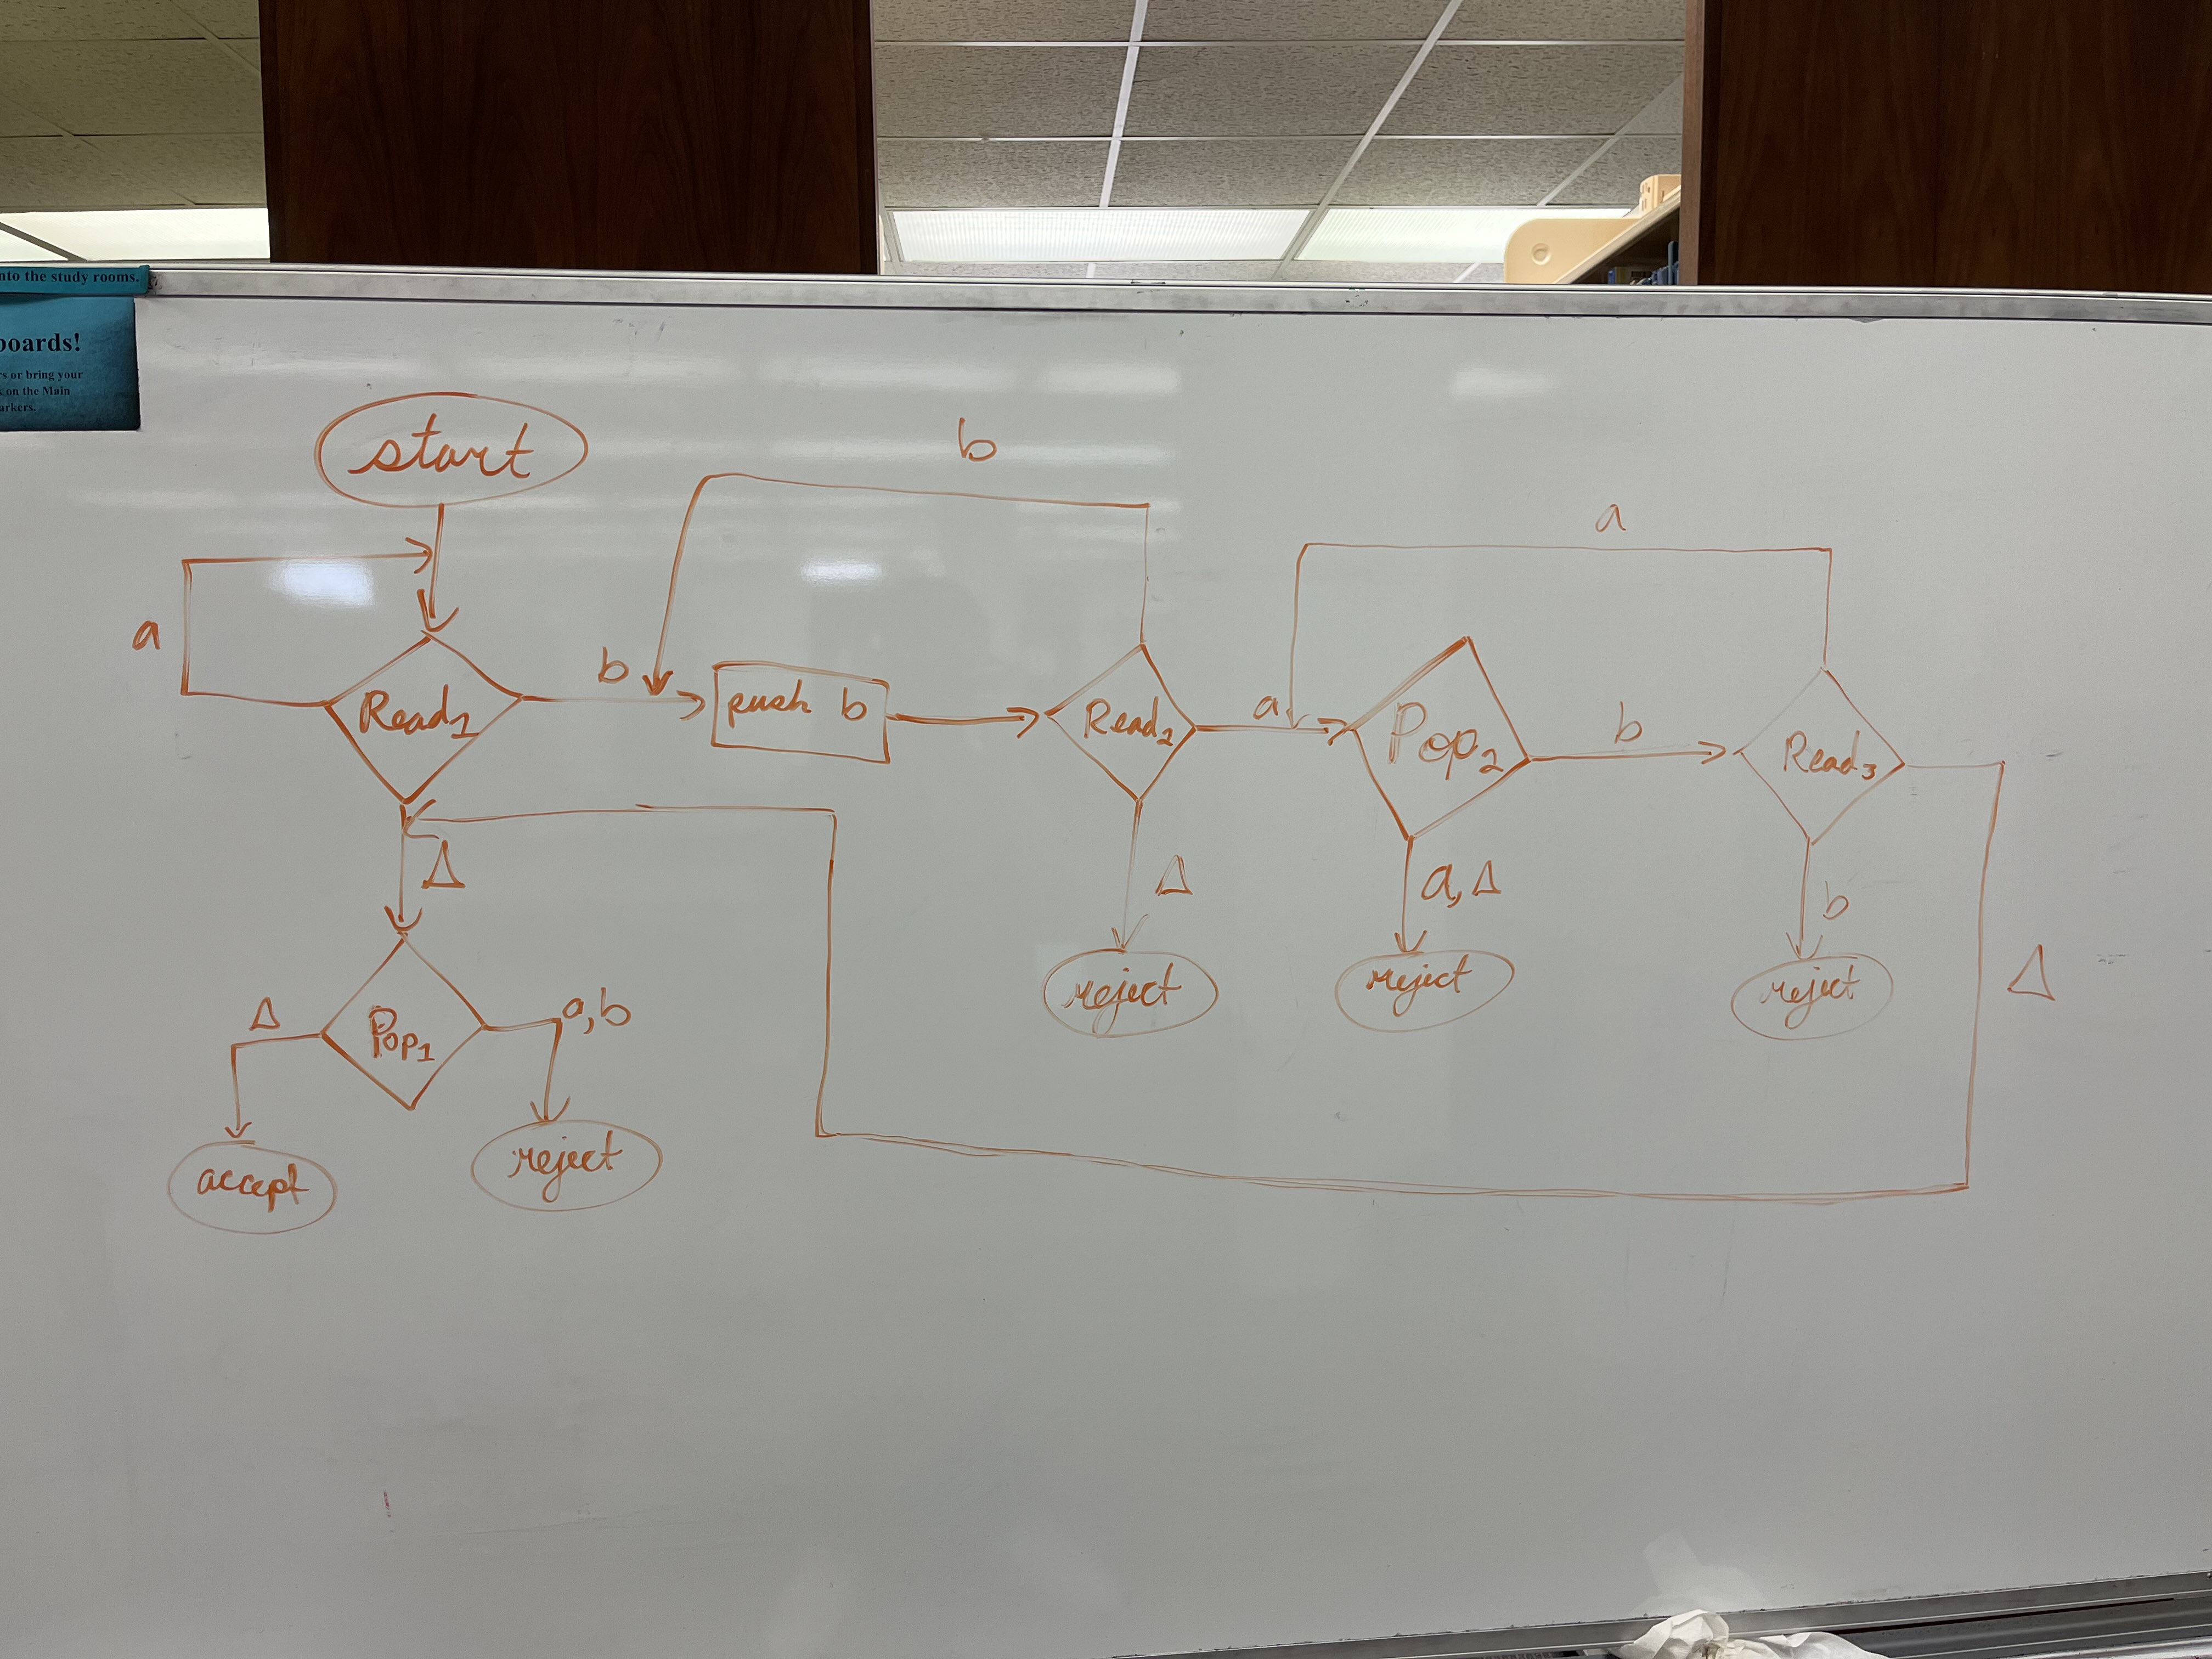
\includegraphics[width=\linewidth]{hw3-q19.jpg}
\end{enumerate}

\Large \textbf{Lecture 14}

\normalsize

\begin{enumerate}
    \item[20.] Using the algorithm of Chapter 15, create a PDA for the language
        ($a^Nba^N$ for $N\geq 0$). For proper credit, show all your work. \\
        \textbf{ANS:} \\
        Convert $S \to aSa | b$ into CNF. \\
        Step 1: Remove null terminals: No null terminals \\
        Step 2: Remove unit productions: No unit productions \\
        Step 3: Separate terminals and non-terminals:
        \begin{itemize}
            \item $S \to ASA | b$
            \item $A \to a$
        \end{itemize}
        Step 3: Ensure RHS limited to 2 NTs:
        \begin{itemize}
            \item $S \to AS_1 | b$
            \item $S_1 \to SA$
            \item $A \to a$
        \end{itemize}
        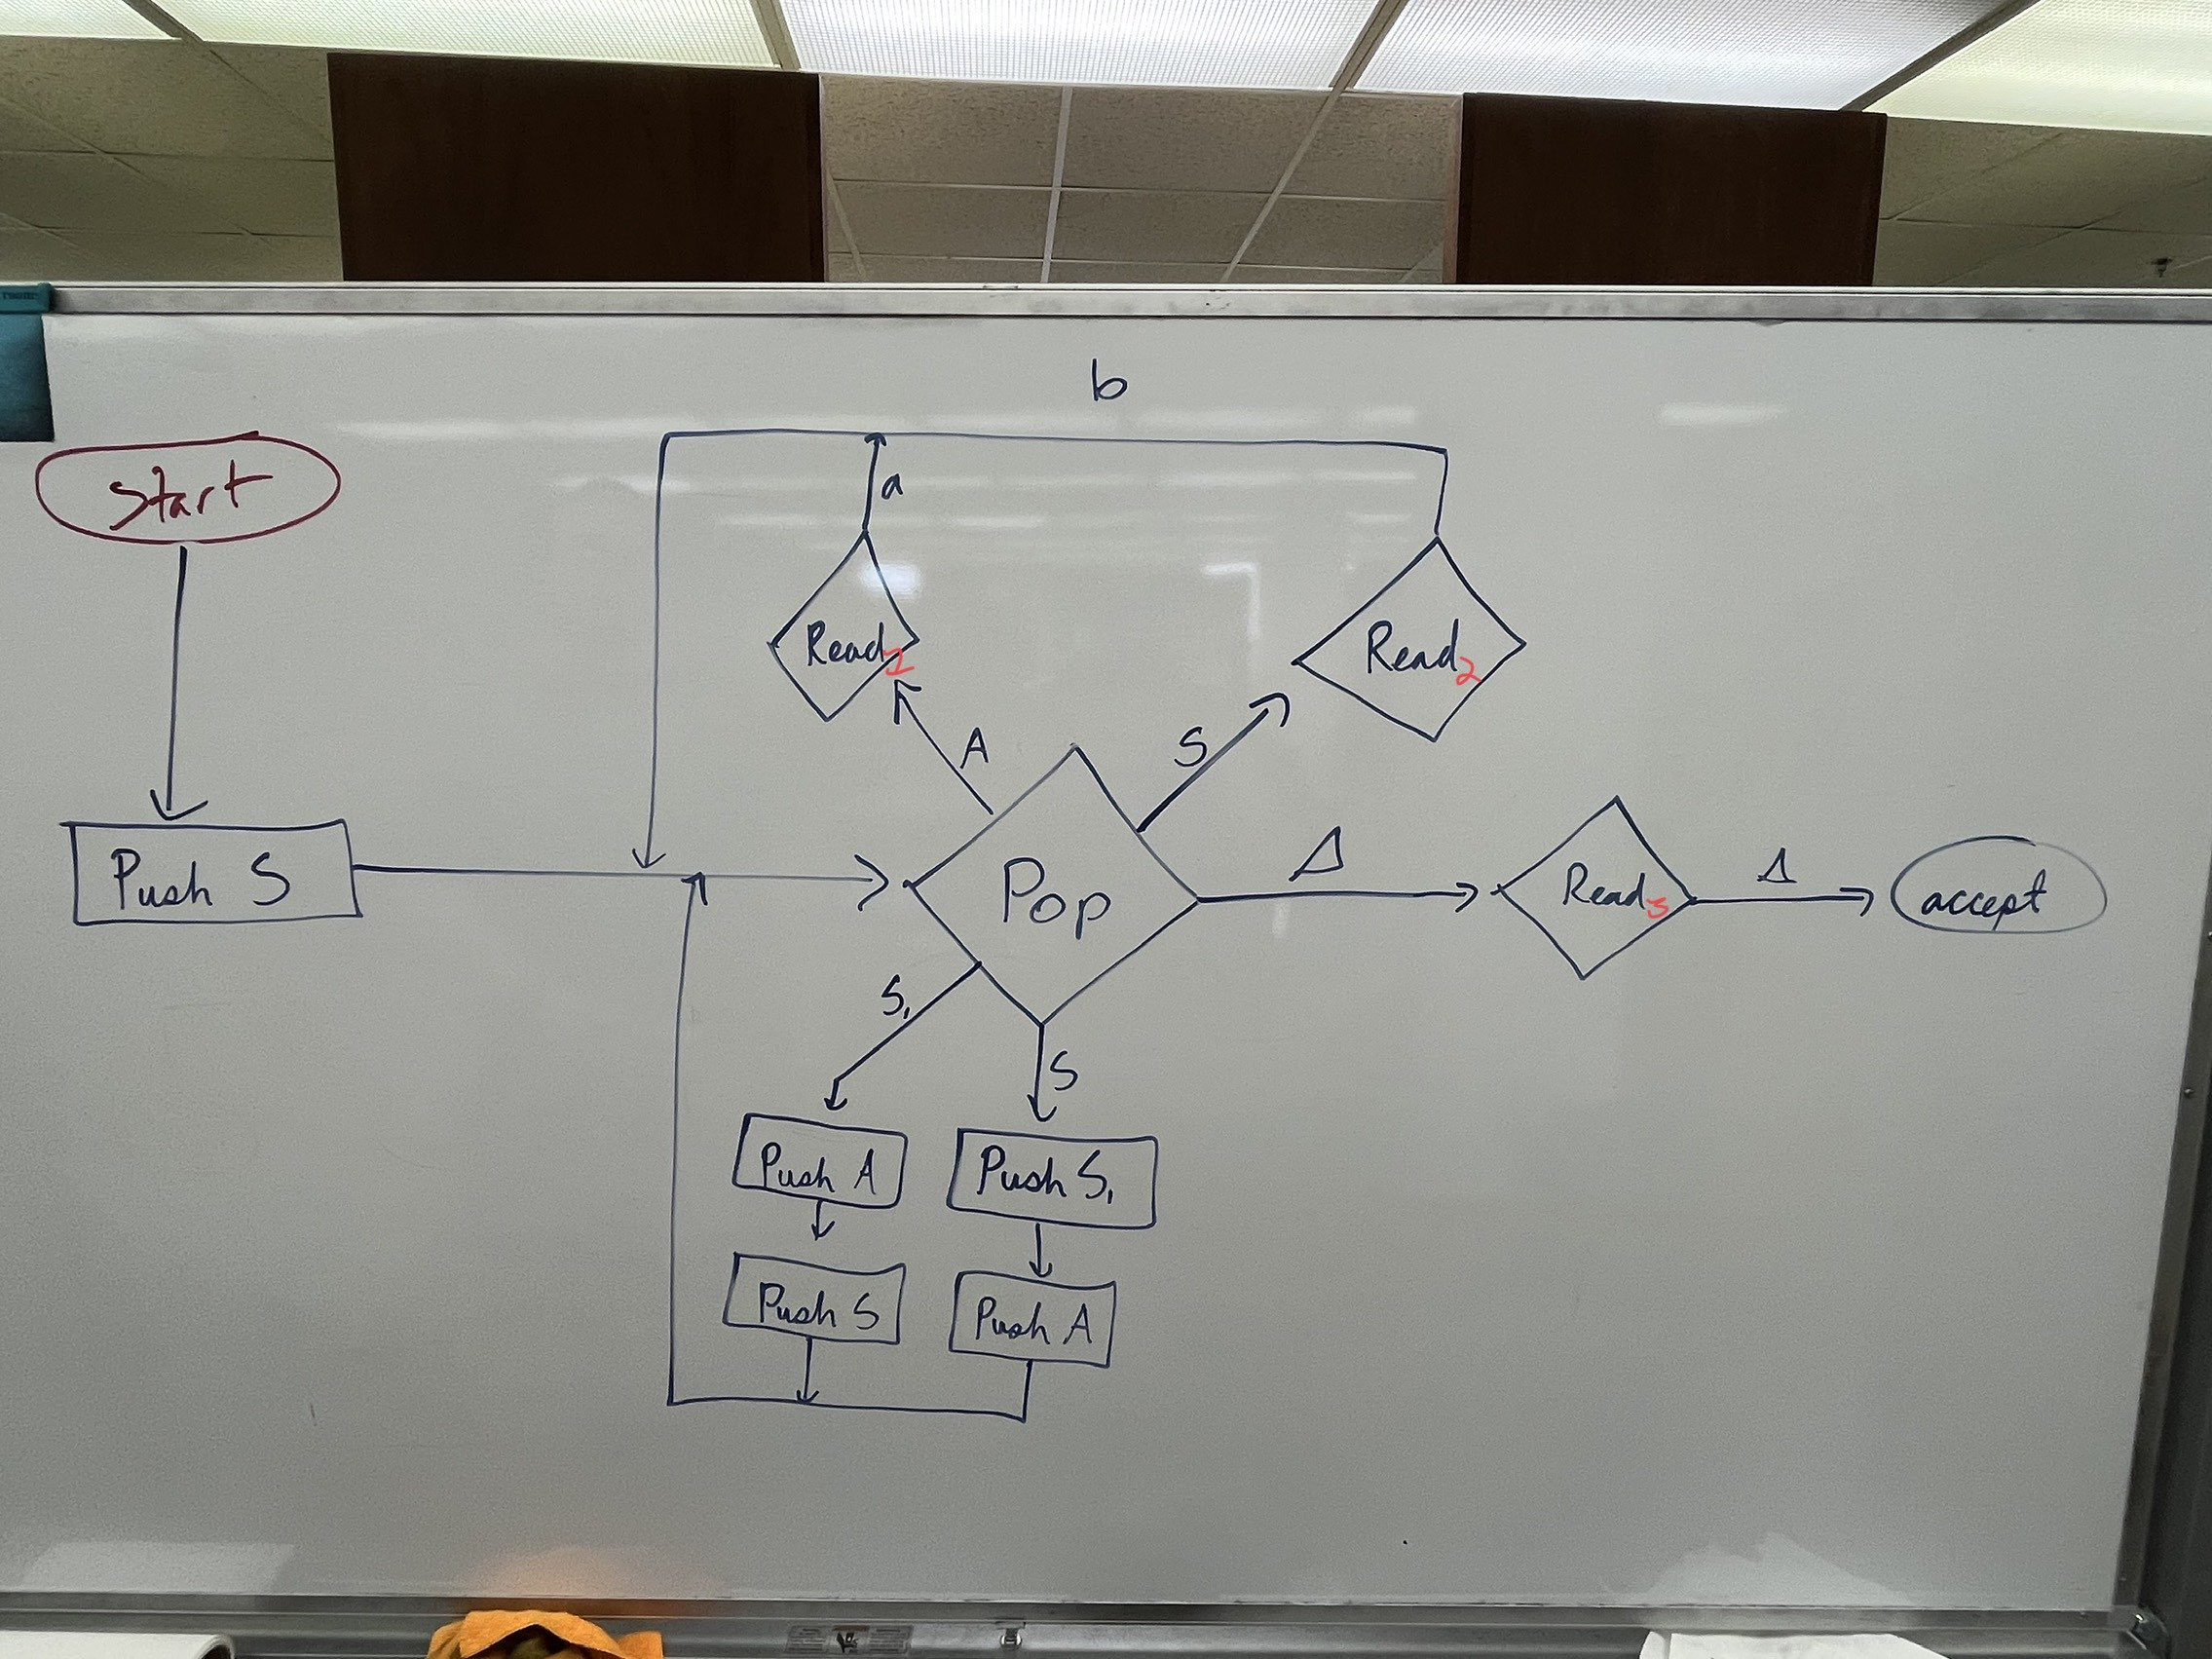
\includegraphics[width=\linewidth]{hw3-q20.jpg}

    \item[21.] Using the approach shown in Slide 10 of this lecture (Lecture
        14), provide a trace through your PDA of the previous problem for the
        word “aabaa”. \\
        \textbf{ANS:} 
        \begin{center}
            \begin{tabular}{| c | c | c | c |}
                \hline
                State      & Stack                                         & Input Tape                                  & Derivation of $aabaa$         \\
                \hline
                Start      & $\Delta \Delta \Delta \Delta \dots          $ & $aabaa               \Delta               $ & \\
                Push S     & $S      \Delta \Delta \Delta \dots          $ & $aabaa               \Delta               $ & \\
                Pop        & $\Delta \Delta \Delta \Delta \dots          $ & $aabaa               \Delta               $ & \\
                Push S$_1$ & $S_1    \Delta \Delta \Delta \dots          $ & $aabaa               \Delta               $ & $S          \implies    AS_1$ \\
                Push A     & $S_1    A      \Delta \Delta \dots          $ & $aabaa               \Delta               $ & \\
                Pop        & $S_1    \Delta \Delta \Delta \dots          $ & $aabaa               \Delta               $ & \\
                Read$_1$   & $S_1    \Delta \Delta \Delta \dots          $ & $\underline{a}abaa   \Delta               $ & $\implies   aS_1$             \\
                Pop        & $\Delta \Delta \Delta \Delta \dots          $ & $aabaa               \Delta               $ & \\
                Push A     & $A      \Delta \Delta \Delta \dots          $ & $aabaa               \Delta               $ & $\implies   aSA$              \\
                Push S     & $A      S      \Delta \Delta \dots          $ & $aabaa               \Delta               $ & \\
                Pop        & $A      \Delta \Delta \Delta \dots          $ & $aabaa               \Delta               $ & \\
                Push S$_1$ & $A      S_1    \Delta \Delta \dots          $ & $aabaa               \Delta               $ & $\implies   aAS_1A$           \\
                Push A     & $A      S_1    A      \Delta \Delta \dots   $ & $aabaa               \Delta               $ & \\
                Pop        & $A      S_1    \Delta \Delta \Delta \dots   $ & $aabaa               \Delta               $ & \\
                Read$_1$   & $A      S_1    \Delta \Delta \Delta \dots   $ & $a\underline{a}baa   \Delta               $ & $\implies   aaS_1A$           \\
                Pop        & $A      \Delta \Delta \Delta \Delta \dots   $ & $aabaa               \Delta               $ & \\
                Push A     & $A      A      \Delta \Delta \Delta \dots   $ & $aabaa               \Delta               $ & $\implies   aaSAA$            \\
                Push S     & $A      A      S      \Delta \Delta \dots   $ & $aabaa               \Delta               $ & \\
                Pop        & $A      A      \Delta \Delta \Delta \dots   $ & $aabaa               \Delta               $ & \\
                Read$_2$   & $A      A      \Delta \Delta \Delta \dots   $ & $aa\underline{b}aa   \Delta               $ & $\implies   aabAA$            \\
                Pop        & $A      \Delta \Delta \Delta \Delta \dots   $ & $aabaa               \Delta               $ & \\
                Read$_1$   & $A      \Delta \Delta \Delta \Delta \dots   $ & $aab\underline{a}a   \Delta               $ & $\implies   aabaA$            \\
                Pop        & $\Delta \Delta \Delta \Delta \Delta \dots   $ & $aabaa               \Delta               $ & \\
                Read$_1$   & $\Delta \Delta \Delta \Delta \Delta \dots   $ & $aaba\underline{a}   \Delta               $ & $\implies   aabaa$            \\
                Pop        & $\Delta \Delta \Delta \Delta \Delta \dots   $ & $aabaa               \Delta               $ & \\
                Read$_3$   & $\Delta \Delta \Delta \Delta \Delta \dots   $ & $aabaa               \underline{\Delta}   $ & \\
                Accept     & $\Delta \Delta \Delta \Delta \Delta \dots   $ & $aabaa               \Delta               $ & \\
                \hline
            \end{tabular}
        \end{center}

    \item[22.] Prove that each of the following languages are Context Free by
        providing Context Free Grammars for each. The grammars do NOT need to be
        in Chomsky Normal Form:
        \begin{enumerate}
            \item[15.1] Language($a^Nb^{2N}$ with $N\geq 0$) \\
                \textbf{ANS:} 
                \begin{itemize}
                    \item $S \to aSbb | \Lambda$
                \end{itemize}
            \item[15.2] Language($a^Nb^Ma^{N+M}$ with $M,N\geq 0$) \\
                \textbf{ANS:} 
                \begin{itemize}
                    \item $S \to aSa | T$
                    \item $T \to bTa | \Lambda$
                \end{itemize}
            \item[15.3] Language($a^Nb^Na^Mb^M$ with $M,N\geq 0$) \\
                \textbf{ANS:} 
                \begin{itemize}
                    \item $S \to AB$
                    \item $A \to aAb | \Lambda$
                    \item $B \to aBb | \Lambda$
                \end{itemize}
        \end{enumerate}

    \item[23.] Using slides 18, 21, and 22 as a guide, show that the Pumping
        Lemma for Context Free Languages holds true for Language ($a^Nb^{2N}$
        with $N\geq 0$). As I did in my examples, the word you build a parse
        tree for doesn’t have to meet the length restriction, as long as you can
        still illustrate the repeating tree descended non-terminal and show U,
        V, X, Y, and Z. \\
        \textbf{ANS:}
        \begin{align*}
            U &= \Lambda \\
            V &= a^{2^P} \\
            X &= abb \\
            Y &= b^{2^P}b^{2^P} \\
            Z &= \Lambda \\
        \end{align*}

        $UV^NXY^NZ \in L \forall N \geq 0$
\end{enumerate}

\end{document}
